\documentclass{beamer}
\usepackage{hyperref}
\usepackage{tikz} 

% Setup appearance:

\usetheme{AnnArbor}
\usecolortheme{beaver}
\usetikzlibrary{arrows,shapes}
\tikzstyle{every picture}+=[remember picture] 

\newcommand{\resitem}[1]{\item \footnotesize {#1} \vspace{0pt}}
\newcommand{\resheading}[1]{{\large {\begin{minipage}{\textwidth}{\textbf{#1 \vphantom{p\^{E}}}}\end{minipage}}}}

\newcommand{\ressubheading}[4]{
\begin{tabular*}{4.4in}{l@{\extracolsep{\fill}}r}
		
		\textbf{#1} & \scriptsize{#2} \\
		\textit{#3} & \scriptsize{\textit{#4}} \\

\end{tabular*}\vspace{-6pt}}


\title{Me}
\author{Gong Li}
\date{January 17, 2014}

\begin{document}
	\begin{frame}{Me - Gong Li}
		\begin{itemize}
		\item
			\ressubheading{Nanyang Technological University}{Singapore}{B.Eng (Hons) in Computer Engineering}{Sep 2010 - May 2014}
			\begin{itemize}
				\resitem {Current GPA \textbf{4.67} on a scale of 5.0, on track of \textbf{First Class Honours} degree}
				\resitem {Awarded the MOE-GLC PRC Undergraduate \textbf{Scholarship} provided by MOE}
				\resitem {Invited to join the \textbf{ELITE+} program by Infocomm Development Authority}
			\end{itemize}

		\item Passionate in \textcolor{red}{Tech}\textcolor{cyan}{nology}
			\begin{itemize}
			\item Final Year Project, Visual Event Recognition in Videos
			\item Summer Research Intern at IBM Research Collaboratory
			\item Face Recognition Project for Machine Learning Course
			\item Android Application with Cloud Assisted
			\end{itemize}
		\end{itemize} 
	\end{frame}

\begin{frame}{Visual Event Recognition}
\begin{itemize}
	\item Goal - recognize various videos based on their content
\end{itemize}

                \begin{tikzpicture}
                        \node (video) at (-1, 0) {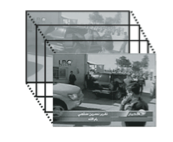
\includegraphics[scale=0.4]{videoSample.png}};
                        \node (videoSIFT) at (2.5,0) {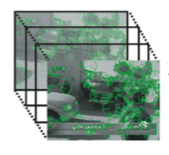
\includegraphics[scale=0.38]{videoSIFT.png}};

                        \draw[->, line width = 2pt, black] (video) -- (videoSIFT) node[pos=.5, above] {\scriptsize{Locate}};

                        \node (SIFTs) at (6,0) {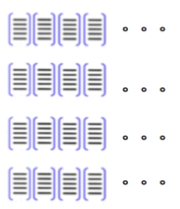
\includegraphics[scale=0.4]{SIFTs}};
                        \draw[->, line width = 2pt, black] (videoSIFT) -- (SIFTs) node[pos=.5, above] {\scriptsize{Describe}};

                        \node (his) at (9, 0) {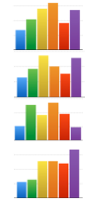
\includegraphics[scale=0.4]{his}};
                        \draw[->, line width = 2pt, black] (SIFTs) -- (his) node[pos=.5, above] {\scriptsize{Project}};

                \end{tikzpicture}

                \begin{columns}
                        \column{0.48\textwidth}
                                \begin{itemize}
                                        \item $M$: number of sampled frames
                                        \item $V$: size of visual vocabulary 
                                \end{itemize}
                        \column{0.6\textwidth}

                                \[
                                          \left(\begin{array}{*5{c}}
                                                   A_{11} & A_{12} & \cdots & \tikz[baseline]{\node[anchor=base] (t1) {$A_{1(V-1)}$};} & A_{1V}\\
                                                A_{21} & A_{22} & \cdots & A_{2(V-1)} & A_{2V}\\
                                                \vdots & \vdots & \vdots & \vdots & \vdots\\
                                                A_{M1} & A_{M2} & \cdots & A_{M(V-1)} & A_{MV}\\
                                          \end{array}\right)
                            \]

            \end{columns}

                \begin{tikzpicture}[overlay]

                        \draw[->, line width = 2pt] (his) -- (t1); 

                \end{tikzpicture}
\end{frame}

\begin{frame}{Projects at IBM}
	\begin{columns}
		\column{0.5\textwidth}{\textbf{Singapore food analysis}}
			\begin{itemize}
				\item Tweets posted in Singapore for 2 years - 20 GB
				\item Most popular food
				\item Sentiment analysis on tweets
				\item Average meal time
				\item Most popular restaurants
			\end{itemize}

           \begin{figure}[!ht]
            \centering
                    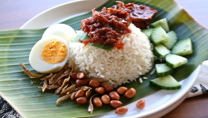
\includegraphics[scale=0.6]{./nasi.png}
            \end{figure}
		
		\column{0.5\textwidth}{\textbf{IBM Connections}}
			\begin{itemize}
				\item Goal - Summarize communities on IBM Connections
				\item Designed a MySQL database
				\begin{figure}[!ht]
		            \centering
		                    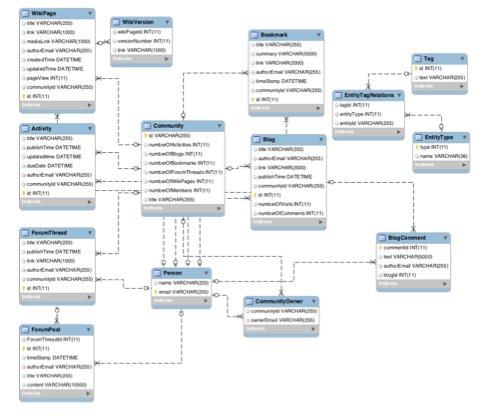
\includegraphics[scale=0.2]{./database.png}
		        \end{figure}

		        \item Implemented 3 algorithms to perform summarization tasks
			\end{itemize}
	\end{columns}
\end{frame}

\begin{frame}{Example on Summarization}
           \begin{figure}[!ht]
            \centering
                    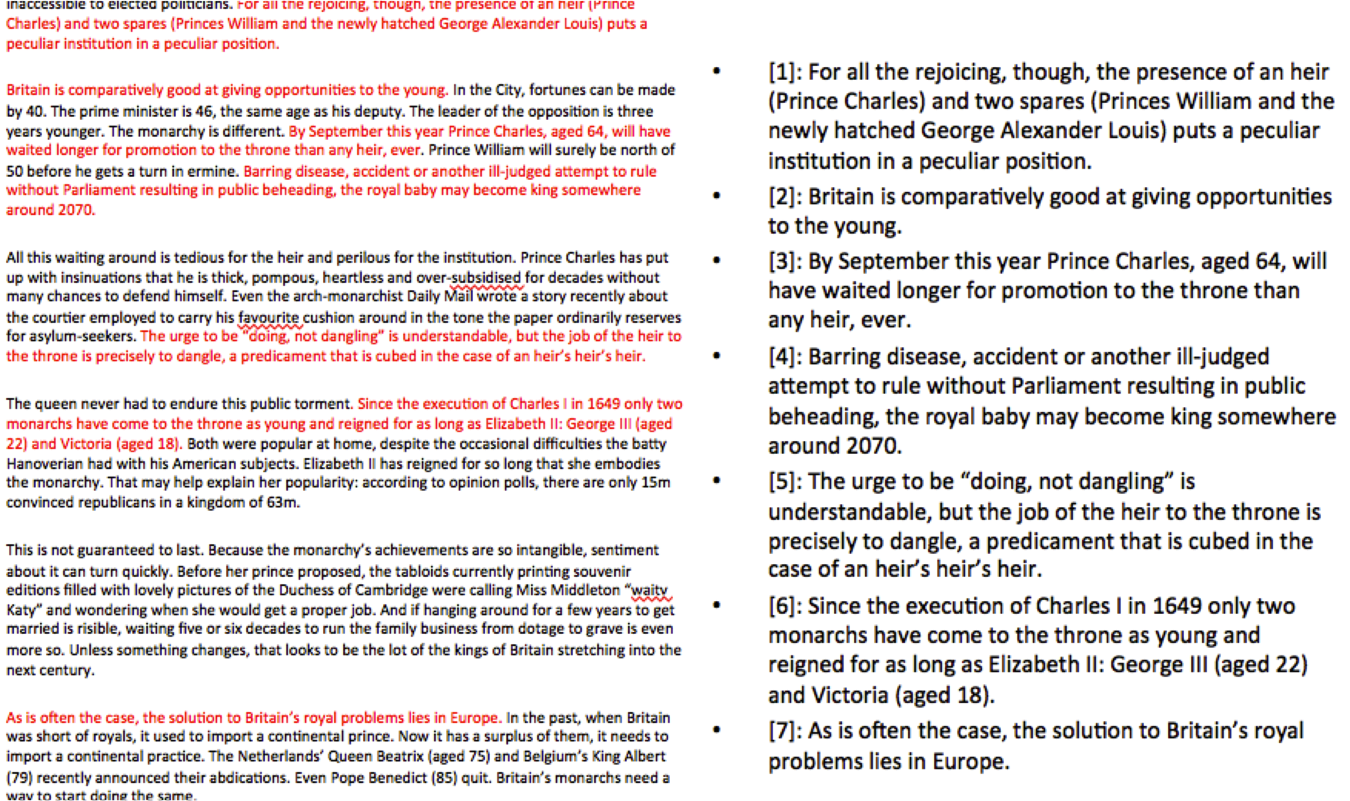
\includegraphics[scale=0.5]{./summarization.png}
            \end{figure}
\end{frame}

\begin{frame}{Face Recognition}
	\begin{itemize}
		\item {Developed a face recognition system in Java based on machine learning knowledge}
		\item {Implemented three different methods: \alert{Eigenfaces, Fishfaces and Laplacianfaces}}
	\end{itemize}
	
	\begin{figure}[!ht]
     	\centering
        	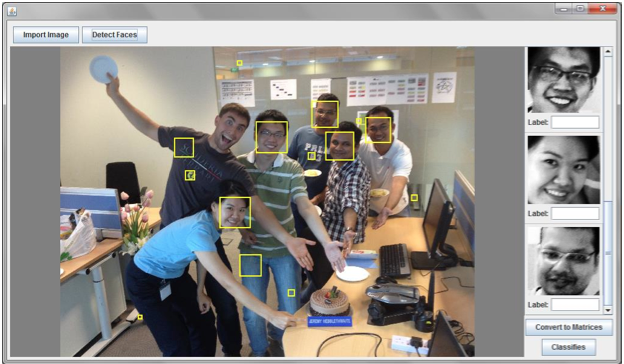
\includegraphics[scale=0.4]{./face.png}
    \end{figure}
\end{frame}

\begin{frame}{Android Application with Cloud Assisted}
	\begin{itemize}
		\item {Developed an android mobile application with cloud assisted}
		\item {Adopted XMPP as the chatting protocol and Youtube as the content}
		\item {Awarded as NTU President \textbf{Research Scholar}}
	\end{itemize}

		\begin{figure}[!ht]
     	\centering
        	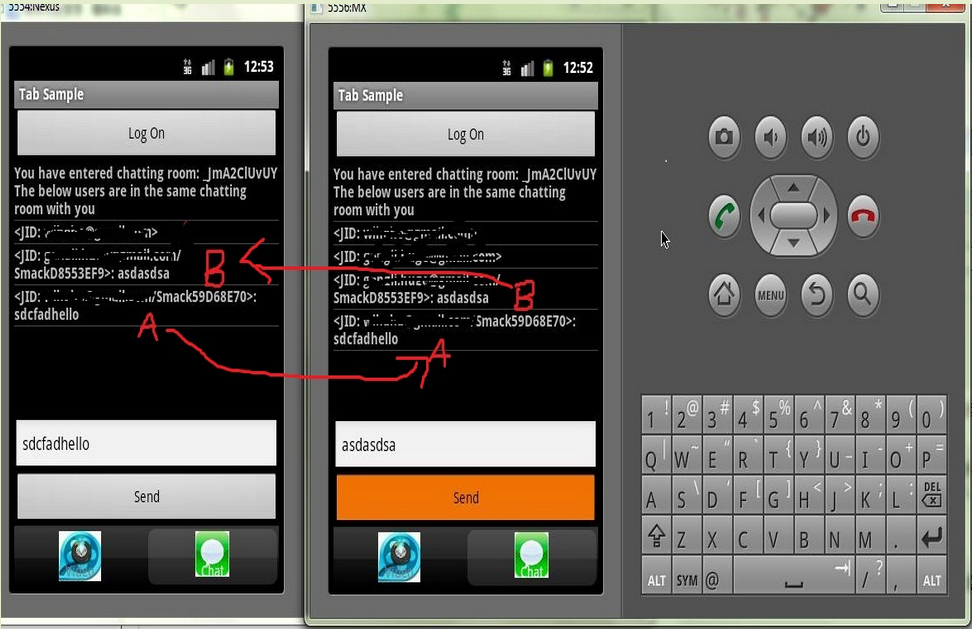
\includegraphics[scale=0.18]{./android.png}
    	\end{figure}
\end{frame}

\begin{frame}
	\begin{center}
		\Large{All personal projects are open sourced on Github}
		\url{https://github.com/wihoho}
	\end{center}

			\begin{figure}[!ht]
     	\centering
        	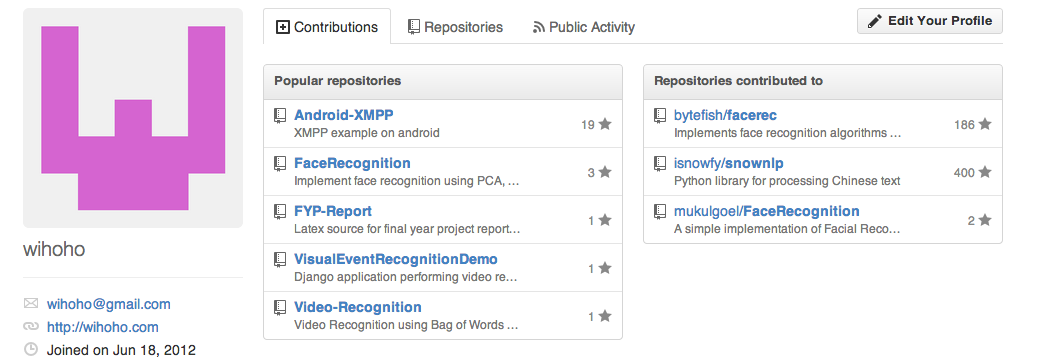
\includegraphics[scale=0.3]{./github.png}
    	\end{figure}
\end{frame}
\end{document}